\documentclass[12pt]{udpreport}
\title{Tarea 1 - Sistema Distribuidos}
\author{
  Gonzalo Gaete Faúndez
  \\
  gonzalo.gaete1@mail.udp.cl
  \\
  Alan Toro Quilaqueo\\
  alan.toro@mail.udp.cl
}

\setlogo{EITFI}

\begin{document}
\maketitle
\tableofcontents
\newpage
\section{Introducción}
El crecimiento acelerado de las ciudades ha generado un aumento significativo en la complejidad de la movilidad urbana, convirtiendo la gestión del tráfico en un desafío global para las autoridades municipales y regionales. El incremento del parque automotor, sumado a una infraestructura vial limitada, demanda el desarrollo de sistemas inteligentes capaces de extraer, procesar y analizar grandes volúmenes de información en tiempo real para optimizar la planificación y la toma de decisiones.

En este contexto, el presente proyecto propone el diseño de una plataforma regional basada en datos colaborativos proporcionados por Waze, con el objetivo de apoyar a la Unidad de Control de Tránsito (UCT) y a las municipalidades en la gestión del tráfico en la Región Metropolitana de Santiago. La solución será desarrollada de forma modular, asegurando su escalabilidad y capacidad de adaptarse a otras regiones en el futuro.

La entrega actual se enmarca en la primera fase del proyecto, denominada \textbf{Datos y Caché}, cuyo propósito es sentar las bases para la recuperación y manejo eficiente de los datos/eventos provenientes de Waze. Esta etapa contempla la automatización del scraping de eventos de tráfico, el diseño de un sistema de almacenamiento capaz de manejar grandes volúmenes de datos de forma ágil, la implementación de un generador de tráfico simulado basado en distribuciones estadísticas y el desarrollo de un sistema de caché parametrizable para optimizar el acceso a los datos más solicitados.

La correcta implementación de esta fase resulta fundamental para garantizar la solidez y el rendimiento del sistema en las etapas posteriores de procesamiento y visualización de información.

\section{Objetivos}
\begin{itemize}
    \item Implementar scraper de eventos Waze.
    \item Diseñar sistema de almacenamiento eficiente.
    \item Construir generador de tráfico usando diferentes distribuciones.
    \item Desarrollar sistema de caché con diferentes políticas de remoción.
    \item Analizar el desempeño del sistema.
\end{itemize}

\section{Arquitectura del Sistema}

La arquitectura consiste en 1 contenedor con el scrapper, 1 contenedor con el almacenamiento, 1 contenedor por cada par de distribución y política de remoción para generar tráfico (4 contenedores total) y lo mismo para las instancias de caché, una por cada par de distribución y política de remoción (4 en total).
\bigskip
Para crear un sistema repetible, cada vez que se levanta el sistema ejecuta todas las combinaciones buscadas. Es decir, en vez de levantar 1 instancia de generador de tráfico y 1 instancia de Redis a la vez con distintas configuraciones. Siempre se levantan todas.

\begin{figure}[h]
    \centering
    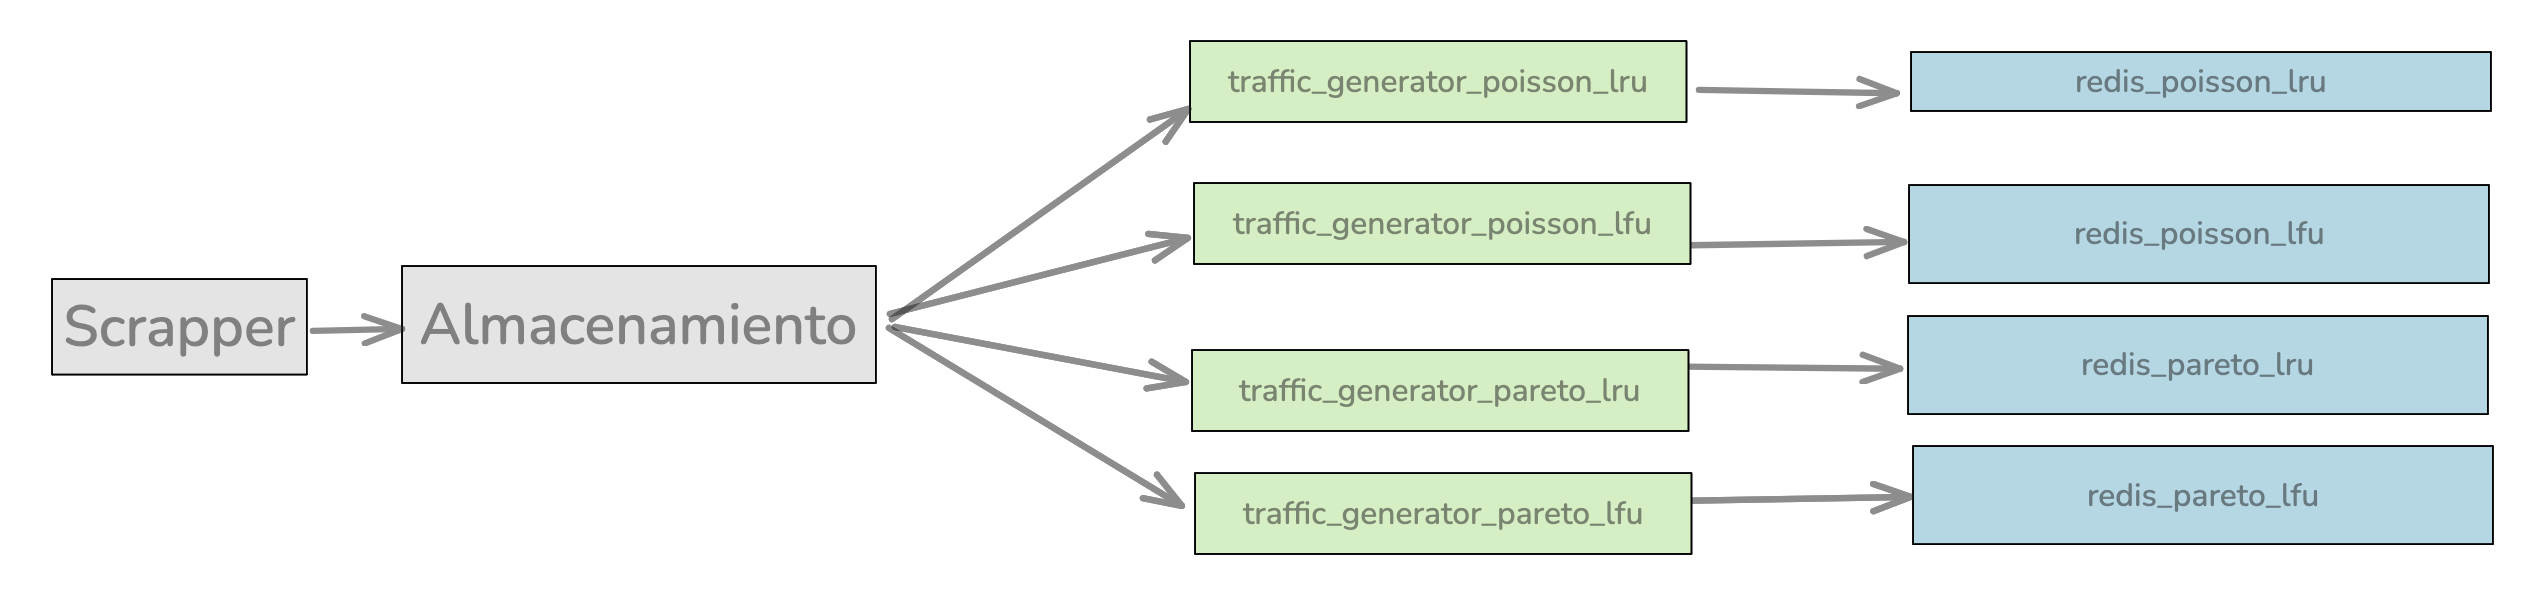
\includegraphics[width=12cm]{images/01-docker-compose.png}
    \caption{Arquitectura del sistema}
\end{figure}

Las razones para las elecciones de tecnología son:

\begin{itemize}
    \item \textbf{Scraper:} Para el scrapper se decidió usar Python por la madurez de las librerías de scrapping y procesamiento de datos. Como también, por su rapidez y simpleza para prototipar proyectos.
    \item \textbf{Almacenamiento: } Para el almacenamiento directo de los eventos se usó MongoDB porque permite trabajar con datos no estructurados de manera rápida y eficiente.
    \item \textbf{Generador de Tráfico: } También se usó Python para el generador de tráfico para mantener un único lenguaje en todo el sistema. Se recibe como variable de entorno la distribución a utilizar (solo dos implementadas: Poisson y Pareto) y la política de remoción para generar logs (solo dos implementadas: LRU y LFU)
    \item \textbf{Sistema de caché: } Para el sistema de caché se decidió usar Redis porque es la base de datos de llave-valor ("key-value database") más popular. Además es configurable mediante variables de entorno lo que facilita parametrizar.
\end{itemize}

\section{Análisis y Discusión}

\subsection{Generador de Tráfico}

Las distribuciones escogidas son \textbf{Poisson} y \textbf{Pareto} para simular la llegada de peticiones. Se elige Poisson porque modela eventos independientes que ocurren con una tasa promedio constante y con una tasa promedio constante en el tiempo, como lo harían los usuarios al consultar información de tráfico. Asi mismo, se elige Pareto para simular casos donde un pequeño porcentaje de eventos genera la mayor cantidad de tráfico (un choque grande en una autopista, puede generar la mayoría del tráfico en un momento dado). Con esto, el generador busca dos casos: un tráfico uniforme con Poisson y un tráfico desbalanceado con Pareto.

\subsection{Almacenamiento}
El sistema de almacenamiento utilizado es \textbf{MongoDB}, la elección se basa en su flexibilidad para manejar datos no estructurados y su buena integración en arquitecturas distribuidas. Permite almacenar datos sin un esquema fijo, lo que facilita el desarrollo iterativo del sistema y presenta tiempos suficientes para que un sistema de caché valga la pena ser implementado. El cuello de botella en este sistema es la lectura en la capa de persistencia con MongoDB. En resumen, es una BBDD fácil de implementar, de integrar en este contexto y genera escrituras rápidas, lecturas "lentas".

\subsection{Cache}
Se utiliza como sistema de caché instancias de Redis con políticas de remoción como \texttt{allkeys-lfu} y \texttt{allkeys-lru}. La elección fue entre las 3 opciones que entrega Redis (LRU, LFU y Random), para tener una intención se eligió LRU (Least Recently Used) que elimina los elementos menos recientemente accedidos y LFU (Least Frequently Used) que favorece los elementos más consultados. Además, se parametriza el tamaño de todas las instancias a 20MB para forzar una gran cantidad de remociones.

\subsection{Métricas}
Las métricas elegidas para incluyen:
\begin{itemize}
    \item \textbf{Hits} y \textbf{misses}, que indican la tasa de aciertos y fallos del caché.
    \item \textbf{Evictions}, que mide cuántos elementos fueron eliminados del caché.
    \item \textbf{Tiempo total de ejecución} y \textbf{tiempo promedio por consulta}, indicadores clave de latencia.
    \item \textbf{Uso de memoria}, que muestra el impacto del sistema en los recursos.
\end{itemize}

\begin{figure}[h]
    \centering
    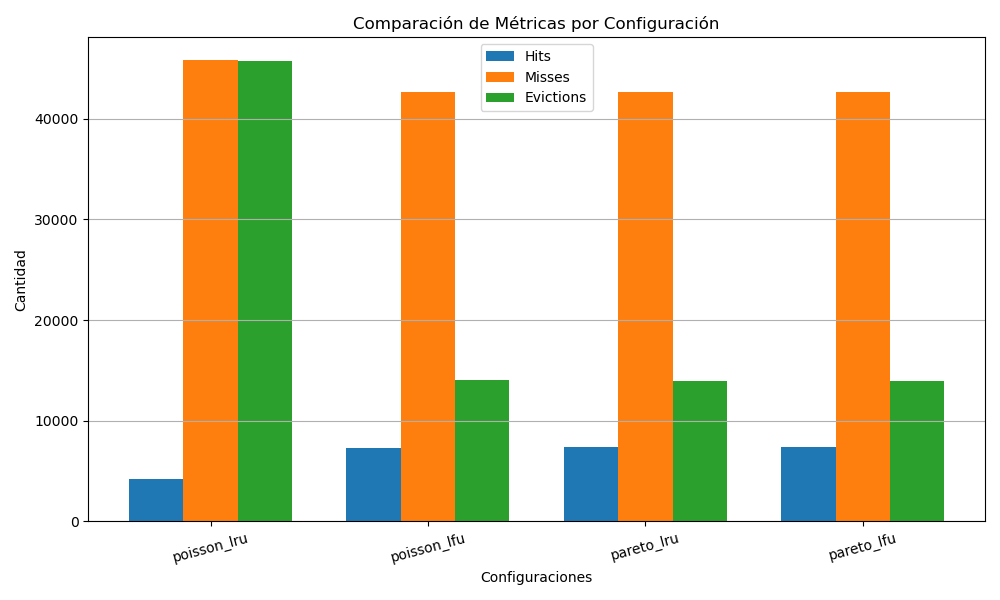
\includegraphics[width=12cm]{images/metricas_comparadas.png}
    \caption{Gráfica de Hit, Misses y Evictions}
\end{figure}

Basado en los datos, la política \texttt{allkeys-lfu} muestra una leve mejora en \textbf{hits} cuando se utiliza con distribución \textbf{Pareto}, lo que sugiere que en sistemas con acceso desigual (como Pareto), esta política es más eficiente.

Además, se aprecia que el \textbf{tiempo promedio por consulta} es menor con la distribución Pareto (0.00209 segundos) respecto a Poisson (0.00240 segundos), lo que indica que la distribución del tráfico tiene un efecto relevante sobre el rendimiento del sistema de caché.

Finalmente, se puede notar cómo el caso de Poisson con LRU es el que tiene la peor proporción de Hit y Misses. El único que se escapa un poco de las tendencias, esto puede ocurrir porque la diversidad de los datos y selección de consultas puede estar dispersa (se repiten pocas consultas "consecutivas").

\subsection{Conclusión}
En el análisis se puede ver que la eficiencia del sistema de caché puede ser relacionada con la política de remoción y la distribución del tráfico. En particular, \texttt{allkeys-lfu} ofrece un mejor rendimiento en escenarios con alta concentración de accesos como los modelados con distribución Pareto. Las métricas utilizadas podrían ser utilizadas para identificar cuellos de botella y evaluar mejoras en la latencia y uso de memoria. Por lo tanto, una correcta elección de política de caché y modelado de tráfico es fundamental para garantizar el rendimiento y la escalabilidad del sistema.


\section{Repositorio}
\noindent Repositorio del proyecto: \\[0.5cm]
\url{https://github.com/wzrdd/SistDist-T1}

\end{document}
